\documentclass[11pt]{article}
\usepackage{arduino-uppgifter}

\newcommand{\mallurl}{https://wokwi.com/projects/357812594927244289}

% Figures subfolder
\graphicspath{{figures/}}

\begin{document}
\begin{center}
      \textbf{\huge{Arduino-övningar}}
      \huge{| MEKMEK01 v11}
\end{center}
\raggedright{}
\begin{center}
      \paddedfbox{
            Nedan kommer några ideer på övningar som kan göras med Arduino. Ni
            kommer att
            ha användning för kunskapen som krävs för att lösa dessa övningar i
            ert
            projektarbete senare i kursen.
      }
\end{center}

\section{Flera blinkande lampor}\label{sec:flera-lampor}
Skapa en krets med 5 lampor, där alla lampor blinkar samtidigt med ett jämnt
intervall, som nedan.
\begin{figure}[H]
      \centering
      \begin{minipage}{0.4\textwidth}
            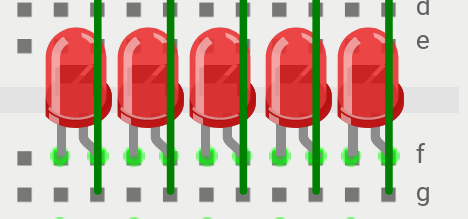
\includegraphics[width=\textwidth]{5led-low}
      \end{minipage}
      \begin{minipage}{0.4\textwidth}
            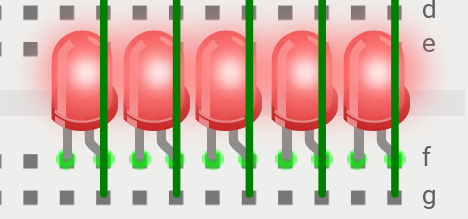
\includegraphics[width=\textwidth]{5led-high}
      \end{minipage}
\end{figure}

\section{Lampor blinkar en-efter-en}\label{sec:sekvensiell-blinkning}
Nu ska lamporna tändas en-efter-en i serie, med jämna mellanrum.
När alla fem lampor har tänts ska alla släckas samtidigt och cykeln börja om.
\begin{figure}[H]
      \centering
      \begin{minipage}{0.3\textwidth}
            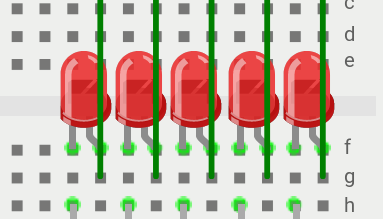
\includegraphics[width=\textwidth]{2-0}
      \end{minipage}
      \begin{minipage}{0.3\textwidth}
            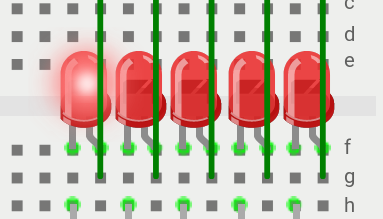
\includegraphics[width=\textwidth]{2-1}
      \end{minipage}
      \begin{minipage}{0.3\textwidth}
            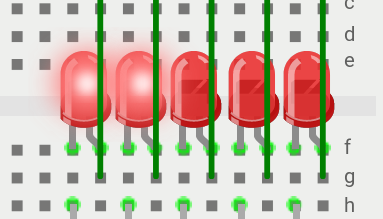
\includegraphics[width=\textwidth]{2-2}
      \end{minipage}
\end{figure}

\section{Multitasking: blinka olika lampor med olika intervall}
\paddedfbox{
      Uppgift \ref{sec:flera-lampor} och \ref{sec:sekvensiell-blinkning} kan lösas
      med \texttt{delay}. Ett problem med den lösningen är att Arduino inte kan göra
      något annat under tiden \texttt{delay} kallas på. Detta kan lösas, genom att
      använda \texttt{millis} och \texttt{if}-satser. Läs på om detta i \href{https://mek.samake.se/arduino/kompendium}{Arduino-kompendiet.}
}

Skapa en krets med 5 lampor, där varje lampa blinkar med olika intervall. Första lampans intervall är 1000ms, andra 500ms, tredje 250ms, fjärde 125ms och femte 62.5ms.

\end{document}